\documentclass[conference]{IEEEtran}
\IEEEoverridecommandlockouts
% The preceding line is only needed to identify funding in the first footnote. If that is unneeded, please comment it out.
\usepackage{cite}
\usepackage{amsmath,amssymb,amsfonts}
\usepackage{algorithmic}
\usepackage{graphicx}
\usepackage{textcomp}
\usepackage{xcolor}
\usepackage{hyperref}
\def\BibTeX{{\rm B\kern-.05em{\sc i\kern-.025em b}\kern-.08em
    T\kern-.1667em\lower.7ex\hbox{E}\kern-.125emX}}
\begin{document}

\title{Field trials using traffic splitting between microservices}

\author{\IEEEauthorblockN{1\textsuperscript{st} Toma Becea}
    \IEEEauthorblockA{\textit{Automation and Computer Science Faculty} \\
    \textit{Technical University of Cluj-Napoca}\\
            Cluj-Napoca, Romania \\
            tomabecea@pm.me}
    \and
    \IEEEauthorblockN{2\textsuperscript{nd} Honoriu Valean}
    \IEEEauthorblockA{\textit{Automation and Computer Science Faculty} \\
    \textit{Technical University of Cluj-Napoca}\\
            Cluj-Napoca, Romania \\
            Honoriu.Valean@aut.utcluj.ro}
}

\maketitle

\begin{abstract}
    When deployments of new versions of a software are needed, their introduction into production might create service disruptions for end users. This papers explores the concept of traffic splitting where a new version is released and then gradually deployed to the users. The graduality means that both versions are up at the same time and the new one will initially receive only 10\% of traffic. If the traffic is deemed to have same error rate as the old version then the splitting rules are increased. Finally, the old version will receive no traffic and can be removed from the system.
\end{abstract}

\begin{IEEEkeywords}
    software trials, microservices, traffic splitting, Kubernetes, Linkerd
\end{IEEEkeywords}

\section{Introduction}
    In today's online software solutions the primary service level agreement (SLA) is the uptime. Site reliability engineers (SREs) are striving to achieve perfection and they measure their target in number of nines, i.e. 99.999\%. Altough for ordinary users the small difference is not noticeable due to their various internet connection problems, the achievement is nevertheless an impresive feat. To achieve this, various tehniques and software solutions are put together in clever ways. This paper will explore the use of microservices for serving traffic and the deployment of new versions of the same software in a manner where users are seeing minimum disruption of the service they are using.

\subsection{Terms}
    To lay the foundation of the upcoming discussion few definitions are needed.
\paragraph{Release}
    The process of release means that a new version of a specific piece of software is running into the production system. However, this new version is not yet serving traffic to external end users.
\paragraph{Deploy}
    Once the new version is starting to serve traffic to external end users, it is said that the version has been deployed.
\paragraph{Error rate}
    A service which responds with error codes, on top of any other data it might need to send back, will likely respond from time to time with codes other than successfull ones (e.g. in HTTP error codes the number 200 means the response is succesfull while the well known number 404 means that a certain resource has not been found), from reasons which are outside its inner workings. For example the users accidentally asks for a resource which was previously deleted, case where the service itself cannot do anything but respond with an error code.

\section{Current state}
    Software deployment has become an area of innovation since CD-ROMs weren't anymore the only solution. One of the old (dated back in 1999) and good readings about this subject propose the Software Dock \cite{b1}. This idea splits the process in two areas: producer side and consumer side. Producer side processes are responsible for bridging the development and deployment realms.

    An interesting read is the analysis made by A. Dearle in \cite{b3}. He analyzes few technology names which were widely used to deploy software, despite the fact that, during the period after \cite{b3} has been published few of those technologies are not anymore the defacto deployment solutions. Java Beans, created by Sun (later it was acquired by Oracle) has 4 phases: development, deployment, service availability and undeployment. Linux is another example using Red Hat Package Manager. Altough RPM is widely in use for deploying software or packages, it is not used to deploy it in live or online environments but rather on linux distros, while in "offline" mode.

    Finally, because this paper mentions error rates, it is worth noting the work of Zhang and Pham, in \cite{b2}, who propose a software reliability growth model and adressing the difference seen between test environment and field environment. The model they propose encompasses the fact that errors and faults are not always solvable in an instant manner but they need to be deferred, usually because of the development process or because of using off-the-shelf software solutions.
    
\section{Solution}

\subsection{Microservices and orchestration}
    Microservices are the state of the art for designing new data and traffic intensive applications, while at the same time taking advantage of few mandatory issues revolving around today's challenges \cite{b5}: security is paramount and isolation and appropiate permissions for them (e.g. no 'sudo' user running code in a container) are an attractive concept. They enable architecture granularity which solves few challenges around Conway's law ("organizations which design systems ... are constrained to produce designs which are copies of the communication structures of these organizations" \cite{b4}). They advertise and mostly provide identical environments for both development and production. They package code and together with a wise package manager (e.g. Node Package Manager or NuGet) they solve the dependency hell and, sometimes, the tight coupling with the host OS (which still exists but is contained in the container as its definition, not anymore a host OS prerequisite). They also provides easier orchestration and elasticity in demand and configuration. However, as much as they are advertised as the ultimate architectural solution, there are cases when different architecture paradigms are better. One example would be monoliths \cite{b6} (altough they are greatly blamed by the proponents of microservices) and another one could be actor model \cite{b7}.

    One can quickly start and use any microservice type approach towards a software solution. Any proof of concept is feasible and doable within minutes with all the open source generally available images for various products (databases, APIs, etc.). However upon doing a commercially viable product or a solution whose complexity is bigger, the first and uttermost problem is the handling of containers. This includes their lifetime, communications between them or with outer entities, persistence, updates, failure resilience, etc. The term "orchestration" sums up all those various operations.
    
    The defacto solution for building and starting containers is Docker \cite{b8}. It also offers a simple orchestrator called Docker Compose, meant to run on a single computer. Its enterprise offerings contain Docker Swarm, a much more capable orchestrator. The current paper, however, will rely on the most ubiquitous solution of today's distributed systems world: Kubernetes \cite{b9}. More details on this, in subsection \ref{subsec:kube}.

\subsection{Kubernetes}
\label{subsec:kube}

    Kubernetes stems from Google and has grown on the experience and challenges Google faced while building and maintaining their services, after two other closed sourced were build and used: Borg and Omega \cite{b9}. Kubernetes is open source and is not anymore managed by Google but by a foundation they have spinned up to oversee Kubernetes (and now they have hundreds of open source solutions in their landscape), called Cloud Native Computing Foundation or CNCF \cite{b11}.

    Its offerings are overwhelming, both in their number and in their complexity. On top of them the third party offerings are intimidating at least. For the current paper only a handful of them will be described.

    Taken in a good order for understanding, the first item to discuss is to asses the microservices concept into Kubernetes context. Being made for orchestrating microservices is itself a collection of various microservices. (The details of its fabric are out of our scope). Therefore whatever it is to run by Kubernetes it has to be an image which became one or more pods (or containers). On top of this we need to know there is a service which knows about all pods of a certain type and expose their ports to outer (within same Kubernetes cluster or outside of it) clients. This service is also an abstraction on top of replicated pods, where it can load balance the traffic or route only to the pods which are healthy. Besides services (and their underpart called deployments) there are many other concepts which are having a play: ingresses, config maps, secrets, replicas, etc.

    The final part for this puzzle we need is the pod mechanics. A pod is the base unit in Kubernetes and it might contain one or more containers. In practice there is a main container which is serving some business logic functionality and all the others, "supporting" containers, are called sidecars. For the current's subject the single piece of interplay between a container and a sidecar, within a pod, is to know the existence of Linux namespaces, specifically of network namespaces \cite{b12}. This functionality allows for a sidecar to hijack the communications of a container, using iptables \cite{b13}, in a transparent manner for the container, i.e. the container do not know that its communications are proxied via a sidecar. In practice this allows for a developer or a devops person to use a self made container with the business functionality it needs, while at the same time to use a third party product for inserting proxy or proxy-based functionalities.

\subsection{Service mesh}

    The high reliance on communications between many microservices has quickly became a friction regarding several aspects. The operational cost of them is one aspect. Then the many layers which a request has to travel or be split into smaller requests makes it difficult to trace it and debug it. Also there are aspects which regard all communications therefore they might benefit of having them centralized and contained. Proxy utilities, for both levels, 4 and 7, are another concern which might have a stake into how a service mesh works. Latencies, HTTP success rates, requests per second, read/write bytes per second, and many others are metrics which need to be looked after. All those aspects and many others, for example see \cite{b15}, come together into an interplay which is generally called a service mesh. One off the shelf product of this type will be used in the implementation, section \ref{sec:implementation}.

\subsection{The concept of traffic splitting}

    \begin{figure}
        \centering
        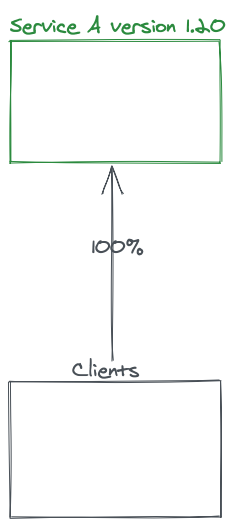
\includegraphics[scale=0.25]{traffic100old.png}
        \caption{Traffic goes to a single version of the service}
        \label{fig:traffic100old}
    \end{figure}

    The departure situation can be seen in figure \ref{fig:traffic100old}. All clients are talking to the same version of the service. It is out of current scope to define the way this traffic goes into a Kubernetes cluster or its ingress, in the its parlance or what kind of traffic is but the assumption is that we have to deal with TCP or UDP traffic, on top of which, usually, there might HTTP calls or RPC ones. The basic assumption, though, is that the proxy which is used is a layer 4 one per Open Systems Interconnection model \cite{b14}.

    \begin{figure}
        \centering
        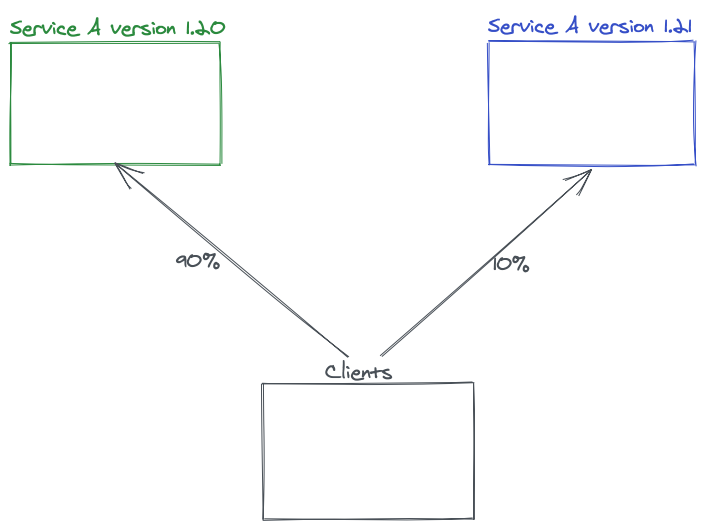
\includegraphics[scale=0.25]{traffic9010.png}
        \caption{Traffic goes to both versions of the service}
        \label{fig:traffic9010}
    \end{figure}

    After the deployment of the new version of the service, the service mesh will start to route a part of the traffic to the new service. Figure \ref{fig:traffic9010} depicts this situation. The factors of routing are a set of initial parameters and they can be manually and progressively modified or an automated tool can be used.

    \begin{figure}
        \centering
        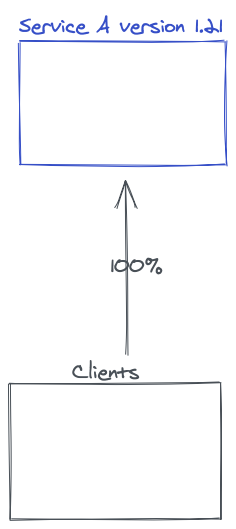
\includegraphics[scale=0.25]{traffic100new.png}
        \caption{Traffic goes to the new version of the service}
        \label{fig:traffic100new}
    \end{figure}

    If the traffic to the new service has the same error rate as the old one and same P99 latency then the finally situation is to have the entire traffic routed only to the new service. This can be seen in \ref{fig:traffic100new}. Once the old service doesn't receive any traffic it can be removed together with all its dependencies.

\section{Implementation}
\label{sec:implementation}

    For the implementation following products have been used: Kubernetes \cite{b9} for orchestrating microservices and Linkerd \cite{b16} as the service mesh. A dummy web server has been setup and an artificial loading pod has been put in place to call the web service and simulate load on it.

    Let's look at the figure \ref{fig:canary}. The service used for rolling its versions is named \textit{podinfo}. The right rectangle, called \textit{svc/podinfo} is the service which internal clients see and can use. External clients may see same service but in order to do this an ingress object has to be set and it has to be instructed to route a certain path towards this service. This ingress become an abstraction which can hide the service name for external clients. Back to the figure \ref{fig:canary}, the right rectangles, called \textit{svc/podinfo-canary} and \textit{svc/podinfo-primary} are the actual two services which correspond to the two versions implied, the old one, named \textit{primary} and new one which the service is rolling to, called \textit{canary}. The same rectangles offers few more informations, in real time:

    \begin{itemize}
        \item Weight is the percent of traffic which is routed to the respective under-service, primary or canary.
        \item SR stands for Success Rate and shows how many requests have succesfully finished.
        \item RPS stands for Requests Per Second
        \item P99 shows the latency for the 99th percentile
    \end{itemize}

    The left rectangle, \textit{svc/podinfo}, shows the SR and RPS numbers in total. As expected, the RPS number for both \textit{primary} and \textit{canary} should sum up to the total.

    Finally, the bottom part of the figure \ref{fig:canary} shows similar information with the difference that it also contains latencies for 50 and 95 percentiles.

    \begin{figure}
        \centering
        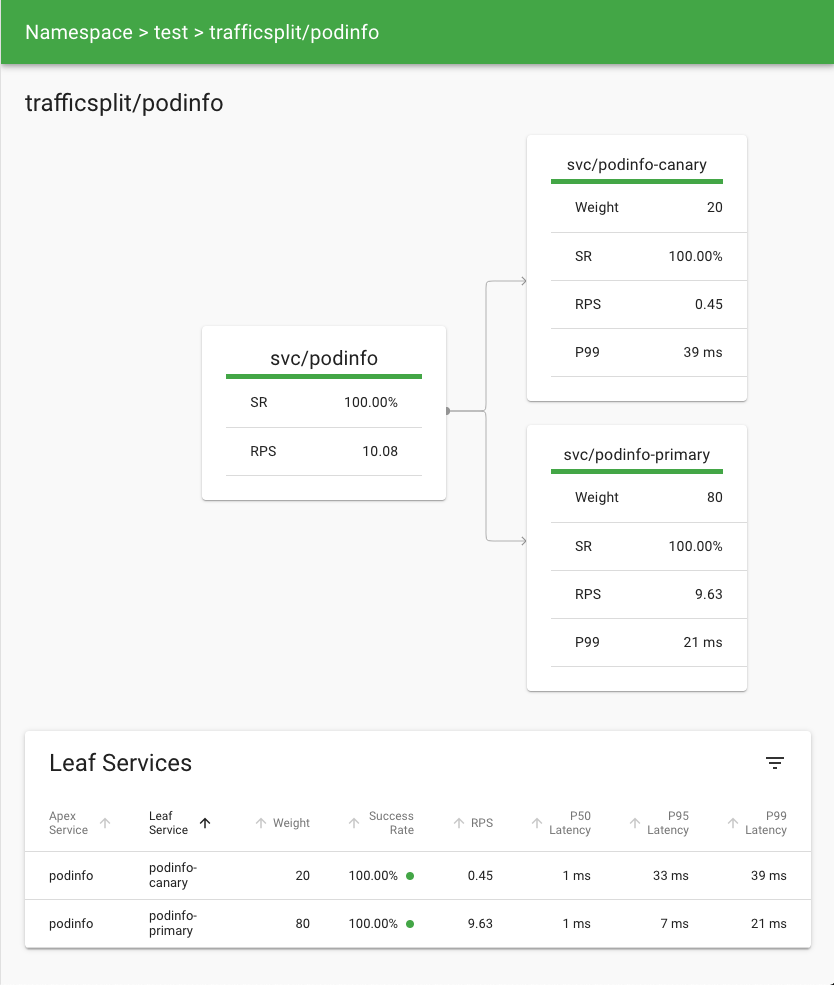
\includegraphics[scale=0.25]{canary.png}
        \caption{Traffic split between two versions}
        \label{fig:canary}
    \end{figure}

    Success rate and latencies are playing a major role into minimizing the errors seen by clients. The rolling process can choose to stop the rolling if the success rate of the canary version drops below 99\% or below the primary version.

\section{Conclusions}

    A generally explanation and few introductory terms have been presented. Also a bit of history of software has been noted through older published papers so that a comparison can be made between what was happening twenty years ago and today. Those have been covered on the \textit{Introduction} and on the \textit{Current state}.
    
    Theoretical and explanatory subjects have been discussed about the world of microservices and orchestration: isolation, containers, orchestration, linux namespaces, communications, proxies and service meshes. Commercial examples have been given so that the concepts discussed can be further studied in the context of how they were implemented.

    The \textit{Solution} section dwells more into how the concepts are choosed to be implemented and what technologies were used, while at the same time offering a complete picture of what traffic splitting is trying to achieve, i.e to minimize the errors seen by the client when new versions of software are deployed and released.

    Finally, the \textit{Implementation} section shows each technology which was choosen and actual screen shots taken during a new software version rolling or releasing, using a service within a Kubernetes cluster.


\begin{thebibliography}{00}

    \bibitem{b1} Hall, Richard S., Dennis Heimbigner, and Alexander L. Wolf. "A cooperative approach to support software deployment using the software dock." Proceedings of the 21st international conference on Software engineering. 1999.

    \bibitem{b2} Xuemei Zhang, Hoang Pham. "Software field failure rate prediction before software deployment, Journal of Systems and Software", Volume 79, Issue 3, 2006, Pages 291-300, ISSN 0164-1212.

    \bibitem{b3} A. Dearle. "Software Deployment, Past, Present and Future," Future of Software Engineering (FOSE '07), Minneapolis, MN, 2007, pp. 269-284. doi: 10.1109/FOSE.2007.20.

    \bibitem{b4} M. Conway, \href{https://en.wikipedia.org/wiki/Conway%27s_law}{Wikpedia, Conway's law page}

    \bibitem{b5} Thones, Johannes. "Microservices." IEEE software 32.1 (2015): 116-116.

    \bibitem{b6} Villamizar, Mario, et al. "Evaluating the monolithic and the microservice architecture pattern to deploy web applications in the cloud." 2015 10th Computing Colombian Conference (10CCC). IEEE, 2015.

    \bibitem{b7} Sheikh, Hammad, Ángel Gómez, and Scott Atran. "Empirical evidence for the devoted actor model." Current Anthropology 57.S13 (2016): S204-S209.

    \bibitem{b8} Docker. \href{https://www.docker.com}{Docker website}

    \bibitem{b9} Kubernetes. \href{https://kubernetes.io}{Kubernetes website}

    \bibitem{b10} Burns, Brendan, et al. "Borg, omega, and kubernetes." Queue 14.1 (2016): 70-93.

    \bibitem{b11} CNCF. \href{https://www.cncf.io}{CNCF website}

    \bibitem{b12} Linux network namespaces. \href{https://www.systutorials.com/docs/linux/man/7-network_namespaces/}{Linux Man Pages}

    \bibitem{b13} Linux IP Tables. \href{https://www.systutorials.com/docs/linux/man/8-iptables/}{Linux Man Pages}

    \bibitem{b14} OSI Model. \href{https://en.wikipedia.org/wiki/OSI_model}{Wikipedia page for OSI Model}

    \bibitem{b15} Li, Wubin, et al. "Service Mesh: Challenges, state of the art, and future research opportunities." 2019 IEEE International Conference on Service-Oriented System Engineering (SOSE). IEEE, 2019.

    \bibitem{b16} Linkerd. \href{https://linkerd.io}{Linkerd website}

\end{thebibliography}
\vspace{12pt}

\end{document}
